\documentclass[a4paper, 12pt]{article}
\usepackage[a4paper, top = 1.5cm, bottom = 1.5cm, left = 1cm, right = 1cm]{geometry}
\usepackage{graphicx}
\usepackage{mathtools}
\usepackage{amsfonts}
\usepackage[english, russian]{babel}
\title{Лабораторная работа № 3.1.3 "Измерение магнитного поля Земли"}
\author{Кирилл Шевцов Б03-402}
\date{8.09.2025}
\begin{document}
\maketitle
\section*{Цель работы}
Исследовать свойства постоянных неодимовых магнитов, с их помощью измерить горизональную и вертикальную составляющую индукции магнитного поля Земли и наклонение.
\section*{Оборудование}
Неодимовые магниты, тонкая нить для изготовления крутильного маятника, медная проволока, электронные весы, секундомер, измеритель магнитной индукции, штангенциркуль.
\section*{Экспериментальная установка}
Для измерения составляющих магнитного поля можно использовать ''магнитную стрелку''. Она образована с помощью $n$ штук намагниченных шариков. Стрелка подвешена в вертикальное положение с помощью $\Lambda-$образного подвеса. Для крепления нити используется штатив, сделанный из немагнитного материала.
\begin{figure}[htbp]
        \centering
        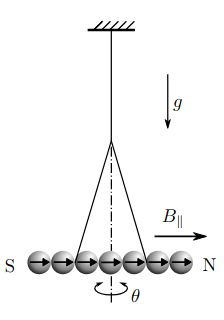
\includegraphics[width=0.25\linewidth]{p1.png}
        \caption{Крутильный маятник во внешнем магнитном поле}
        \label{Подвес}
\end{figure}
\newpage
Измерить магнитное поле Земли можно при помощи силы отрыва шариков от цепочки:
\begin{figure}[htbp]
    \centering
    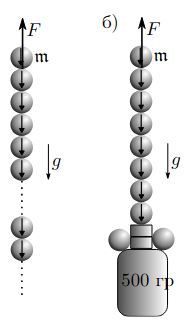
\includegraphics[width=0.25\linewidth]{p2.png}
    \caption{Установка для силы отрыва}
    \label{установка для силы отрыва}
\end{figure}\\
Альтернативным способом иможет быть измерение магнитного момента двух одинаковых шариков заданной массы и радиуса.
Такая установка состоит из немагнитного штатива, с укрепленными перпендикулярно его оси двух платформ, имеющих небольшой вогнутый сферический сегмент
для шариков:
\begin{figure}[htbp]
    \centering
    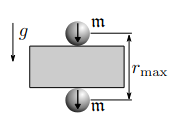
\includegraphics[width=0.25\linewidth]{p3.png}
    \caption{Измерение магнитного момента шариков}
    \label{установка измерение магнитного момента шариков}
\end{figure}
\section*{Необходимые формулы и теория}
\paragraph{}
Простейший магнитный диполь может быть образован витком с током или постоянным магнитом.\\
Магнитное поле точечного диполя вычисляется подобно формуле напряженности электрического поля этого диполя:
\begin{equation}
    \mathbf{B} = \frac{\mu_{0}}{4 \pi}\left(\frac{3({\mathfrak{m}} \cdot \mathbf{r}) \mathbf{r}}{r^{5}} - \frac{{\mathfrak{m}}}{r^{3}}\right)
    \label{Магнитное поле диполя}
\end{equation}
Здесь $\mu_{0} = 4\pi \cdot 10^{-7}$ Гн/м - магнитная постоянная, $\mathbf{\mathfrak{m}}$ - магнитный момент точечного диполя, $\mathbf{r}$ - радиус вектор, направленный от диполя в рассматриваемую точку.\\
Во внешнем магнитном поле с индукцией $\mathbf{B}$ на точечный магнитный диполь $\mathfrak{m}$ действует механический момент сил:
\begin{equation}
    \mathbf{M} = [\mathfrak{m} \times \mathbf{B}]
    \label{Момент}
\end{equation}
В неоднородном магнитном поле на точечный диполь действует сила:
\begin{equation}
    \mathbf{F} = (\mathfrak{m} \cdot \nabla)\mathbf{B}
    \label{Сила действия на диполь}
\end{equation}
В частности, проекция силы на ось $\mathit{Ox}$:
\begin{equation}
    F_{x} = \mathfrak{m}_{x}\frac{\partial B_{x}}{\partial x} + \mathfrak{m}_{y}\frac{\partial B_{x}}{\partial y} + \mathfrak{m}_{z}\frac{\partial B_{x}}{\partial z}
    \label{Проекция силы}
\end{equation}
\paragraph{}
Формулы (\ref{Момент}) и (\ref{Сила действия на диполь}) помогают рассчитать силу взаимодействия магнитов с моментами $\mathfrak{m_{1}}$ и $\mathfrak{m_{2}}$ в рамках точечных диполей:
\begin{equation}
    F_{12} = \mathfrak{m}_{1}{\frac{\partial {B_{2}}}{\partial r}} = \mathfrak{m}_{1}\frac{\partial (2\mathfrak{m}_{2}/r^{3})}{\partial r}  =-6\frac{\mathfrak{m}_{1}\mathfrak{m}_{2}}{r^{4}}
    \label{Сила взаимодействия диполей}
\end{equation}
Для рассчета магнитного поля Земли есть несколько методов:
\begin{enumerate}
    \item Определить магнитный момент $\mathfrak{m}$ двух из шариков, определив наибольшее расстояние $\mathit{r_{max}}$, на котором они смогут удерживать друг друга в поле тяжести. По величине $\mathfrak{m}$\
    с помощью (\ref{Магнитное поле диполя}) рассчитать величину индукции вблизи любой точки на поверхности шара радиусом $\mathit{R}$.
    \begin{equation}
        \mathfrak{m} = \sqrt{\frac{mgr_{max}^{4}}{6}}
        \label{Магнитный момент}
    \end{equation}\\
    Учтем, что здесь магнитный момент представлен вычислением в единицах СГС.
    \item Величину магнитного поля можно определить с помощью силы сцепления намагниченных шариков. Определим ее, как необходимую силу для разрыва двух сцепившихся шариков. Сила сцепления (\ref{Сила взаимодействия диполей}) равна:
    \begin{equation}
        F_{0} = \frac{6\mathfrak{m}^{2}}{(2R)^{4}} = \frac{3\mathfrak{m}^2}{8R^{4}}
        \label{Сила сцепления}
    \end{equation}
    Минимальный вес цепочки, при которой она оторвется от верхнего шарика, равна:
    \begin{equation}
        F = F_{0}\left(\sum_{k = 1}^n \frac{1}{k^{4}}\right) \approx 1,08F_{0}
        \label{Вес цепочки}
    \end{equation}
    Учтём, что сила сцепления шариков при их отрывании убывает как $1/r^{4}$.
    \item Рассчитаем магнитное поле Земли с помощью составляющих: вертикальной и горизонтальной, ведь:
    \begin{equation}
        \mathbf{B} = \mathbf{B_{||}} + \mathbf{B_{\perp}}
        \label{Векторная сумма полей}
    \end{equation}
    Горизонтальную составляющую поля можно рассчитать с помощью измерения периода крутильных колебаний ''магнитной стрелки'' вокруг своей оси:
    \begin{equation}
        T_{n} = 2\pi \sqrt{\frac{mR^{2}}{3\mathfrak{m}B_{||}}}\cdot n
        \label{Период крутильных колебаний}
    \end{equation}
    По зависимости $T(n) = f(n)$, а это прямая, можно определить коэффициент наклона и по нему найти модуль горизонтальной составляющей поля.\\
    Рассчитать вертикальную составляющую поля можно при помощи той же магнитной стрелки. При отклонении стрелки возникает момент силы натяжения нити. Поэтому, можно выровнять положение стрелки, подвесив на некоторое ее расстояние $x$ груз массой $m_{x}$. Отсюда получим выражение для вертикальной составляющей магнитного поля:
    \begin{equation}
        m_{x}gx = n\mathfrak{m}B_{\perp} \iff B_{\perp} = \frac{m_{x}gx}{n\mathfrak{m}}
        \label{Вертикальная составляющая}
    \end{equation}\\
    Здесь полезно рассмотреть зависисмость момента силы тяжести от количества шариков (это набор четных чисел), построить график $\mathcal{M}_{n}(n) = \mathfrak{m} B_{\perp}n$ и уже по его угловому коэффициенту определить нужную составляющую.\\
    Теперь, зная составляющие магнитного поля, можно рассчитать магнитное поле Земли согласно (\ref{Векторная сумма полей}).
\end{enumerate}
\end{document}
